\documentclass[12pt,a4paper]{report}
\usepackage[T1]{fontenc}
\usepackage[utf8]{inputenc}
\usepackage{charter}
\usepackage{ngerman}
\usepackage[left=2cm,right=2cm,top=2cm,bottom=2cm]{geometry}
\renewcommand\thesection{\arabic{section}.}
\usepackage{tikz} 

\begin{document}
	\section*{2.6 Die Hallwachs-Experimente}
	In den Hallwachs-Experimenten wird eine geladene Metallplatte mit Licht einer Quecksilberdampflampe bestrahle:
	\begin{itemize}
		\item[1)] Platte negativ geladen $\to$ Das Licht entlädt die Platte (erkennbar am Zurückgehen des Ausschlags am Elektroskop.)
		\item[2)] Platte positiv geladen $\to$ Keine Entladung erkennbar
		\item[3)] Platte negativ geladen, Glasplatte eingefügt $\to$ keine Entladung erkennbar
	\end{itemize}
	\underline{\textbf{FAZIT}}: Das Licht löst die Elektronen von der Platte ab. \\[1cm]
	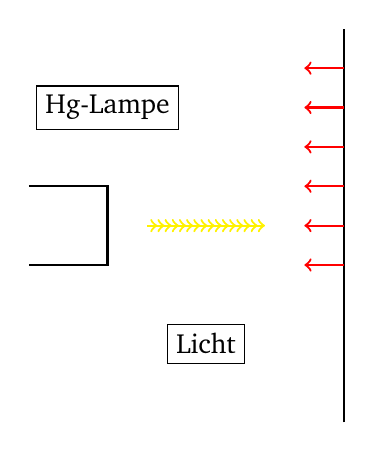
\begin{tikzpicture}
		\draw[thick] (0,1) -- (1,1) -- (1,0) -- (0,0);
		\draw[->>>>>>>>>>>>>>>>,thick,yellow] (1.5,0.5) -- (3,0.5);
		\node[draw] at (1,2) {Hg-Lampe};
		\node[draw] at (2.25,-1) {Licht};
		\draw[thick] (4,-2) -- (4,3);
		\draw[thick,red,->] (4,2.5) -- (3.5,2.5);
		\draw[thick,red,->] (4,2) -- (3.5,2);
		\draw[thick,red,->] (4,1.5) -- (3.5,1.5);
		\draw[thick,red,->] (4,1) -- (3.5,1);
		\draw[thick,red,->] (4,0.5) -- (3.5,0.5);
		\draw[thick,red,->] (4,0) -- (3.5,0);
	\end{tikzpicture}\\
	Der Photoeffekt setzt sofort ein. Nur das (nicht sichtbare) UV-Licht lässt die Elektronen lösen.
	\\
	$\Rightarrow$ Licht ist ein Teilchen?
\end{document}